\documentclass[11pt,a4paper]{report}
\usepackage[textwidth=37em,vmargin=30mm]{geometry}
\usepackage{calc,xunicode,amsmath,amssymb,paralist,enumitem,tabu,booktabs,datetime2,xeCJK,xeCJKfntef,listings}
\usepackage{tocloft,fancyhdr,tcolorbox,xcolor,graphicx,eso-pic,xltxtra,xelatexemoji}

\newcommand{\envyear}[0]{2024}
\newcommand{\envdatestr}[0]{2024-11-18}
\newcommand{\envfinaldir}[0]{webdb/2024/20241118/final}

\usepackage[hidelinks]{hyperref}
\hypersetup{
    colorlinks=false,
    pdfpagemode=FullScreen,
    pdftitle={Web Digest - \envdatestr}
}

\setlength{\cftbeforechapskip}{10pt}
\renewcommand{\cftchapfont}{\rmfamily\bfseries\large\raggedright}
\setlength{\cftbeforesecskip}{2pt}
\renewcommand{\cftsecfont}{\sffamily\small\raggedright}

\setdefaultleftmargin{2em}{2em}{1em}{1em}{1em}{1em}

\usepackage{xeCJK,xeCJKfntef}
\xeCJKsetup{PunctStyle=plain,RubberPunctSkip=false,CJKglue=\strut\hskip 0pt plus 0.1em minus 0.05em,CJKecglue=\strut\hskip 0.22em plus 0.2em}
\XeTeXlinebreaklocale "zh"
\XeTeXlinebreakskip = 0pt


\setmainfont{Brygada 1918}
\setromanfont{Brygada 1918}
\setsansfont{IBM Plex Sans}
\setmonofont{JetBrains Mono NL}
\setCJKmainfont{Noto Serif CJK SC}
\setCJKromanfont{Noto Serif CJK SC}
\setCJKsansfont{Noto Sans CJK SC}
\setCJKmonofont{Noto Sans CJK SC}

\setlength{\parindent}{0pt}
\setlength{\parskip}{8pt}
\linespread{1.15}

\lstset{
	basicstyle=\ttfamily\footnotesize,
	numbersep=5pt,
	backgroundcolor=\color{black!5},
	showspaces=false,
	showstringspaces=false,
	showtabs=false,
	tabsize=2,
	captionpos=b,
	breaklines=true,
	breakatwhitespace=true,
	breakautoindent=true,
	linewidth=\textwidth
}






\newcommand{\coverpic}[2]{
    % argv: itemurl, authorname
    Cover photo by #2~~(\href{#1}{#1})
}
\newcommand{\makeheader}[0]{
    \begin{titlepage}
        % \newgeometry{hmargin=15mm,tmargin=21mm,bmargin=12mm}
        \begin{center}
            
            \rmfamily\scshape
            \fontspec{BaskervilleF}
            \fontspec{Old Standard}
            \fontsize{59pt}{70pt}\selectfont
            WEB\hfill DIGEST
            
            \vfill
            % \vskip 30pt
            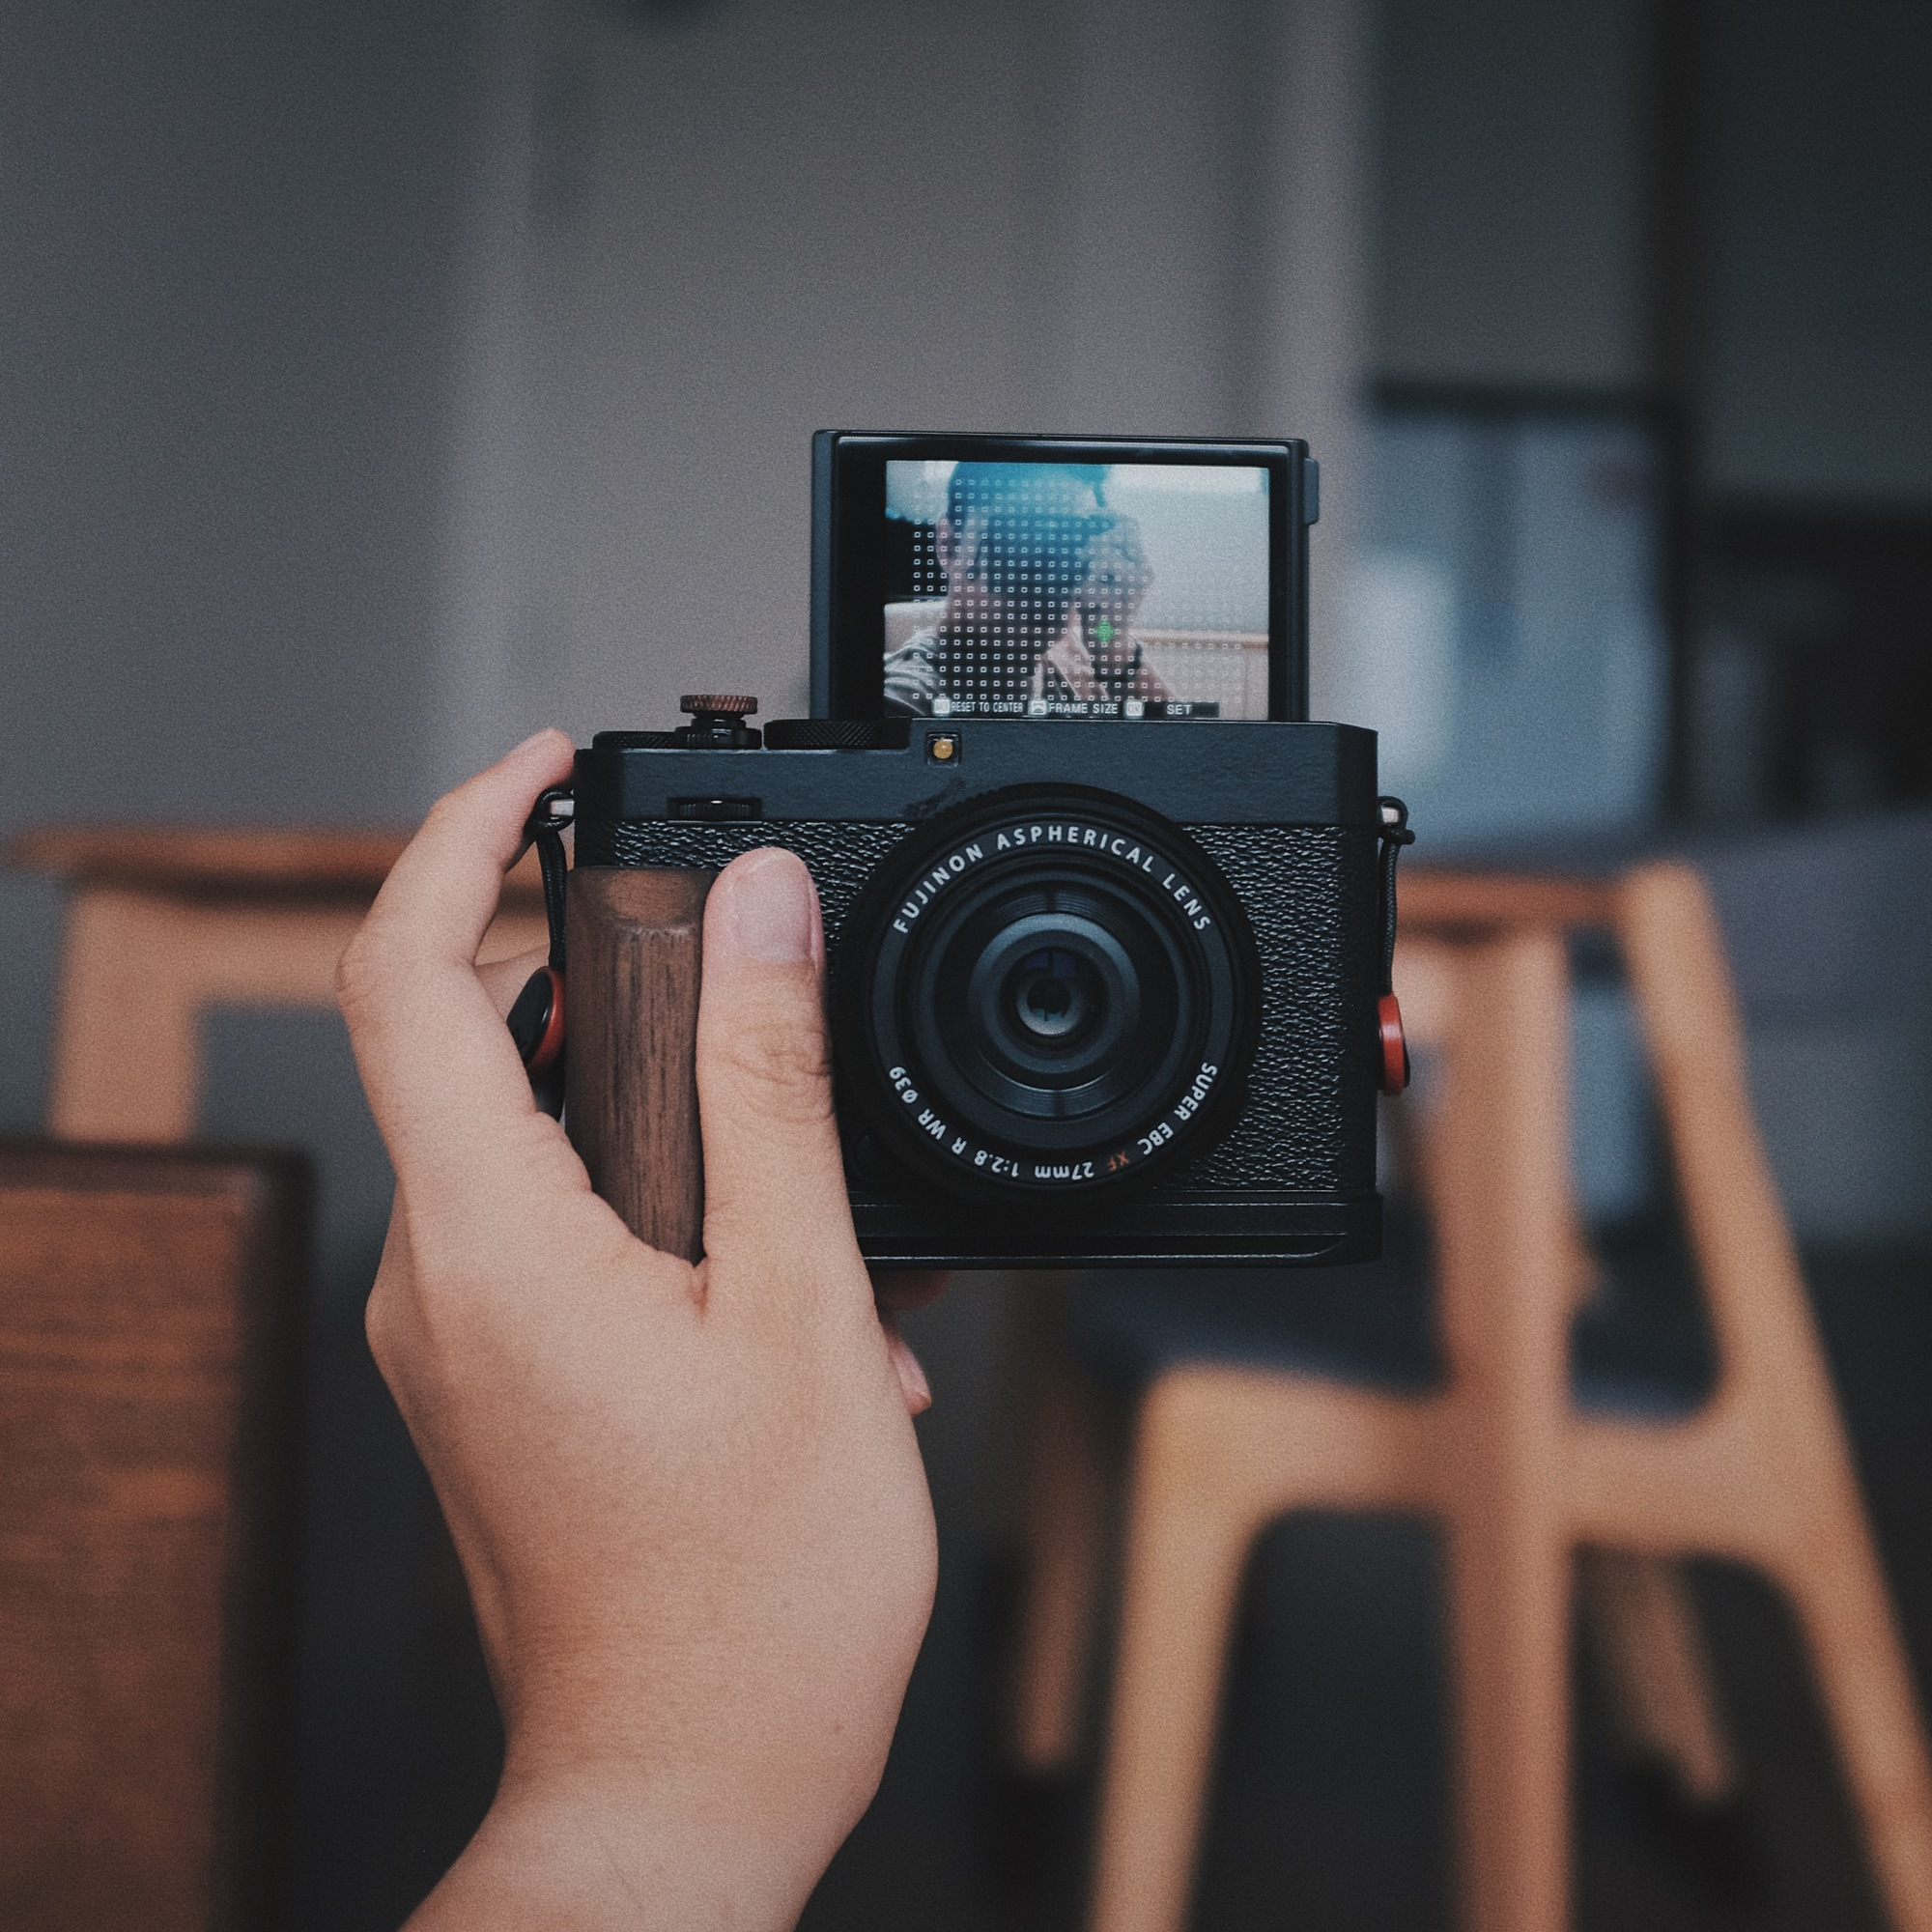
\includegraphics[width=\linewidth]{\envfinaldir/coverpic-prod.jpg}\par
            % \vskip 30pt
            \vfill

            \normalsize\rmfamily\scshape
            \copyright{} The Web Digest Project \hfill\large \envdatestr
        \end{center}
    \end{titlepage}
    % \restoregeometry
}
\newcommand{\simplehref}[1]{%
    \textcolor{blue!80!green}{\href{#1}{#1}}%
}
\renewcommand{\contentsname}{\center\Huge\sffamily\bfseries Contents\par\vskip 20pt}
\newcounter{ipartcounter}
\setcounter{ipartcounter}{0}
\newcommand{\ipart}[1]{
    % \vskip 20pt
    \clearpage
    \stepcounter{ipartcounter}
    \phantomsection
    \addcontentsline{toc}{chapter}{#1}
    % \begin{center}
    %     \Huge
    %     \sffamily\bfseries
    %     #1
    % \end{center}
    % \vskip 20pt plus 7pt
}
\newcounter{ichaptercounter}
\setcounter{ichaptercounter}{0}
\newcommand{\ichapter}[1]{
    % \vskip 20pt
    \clearpage
    \stepcounter{ichaptercounter}
    \phantomsection
    \addcontentsline{toc}{section}{\numberline{\arabic{ichaptercounter}}#1}
    \begin{center}
        \Huge
        \sffamily\bfseries
        #1
    \end{center}
    \vskip 20pt plus 7pt
}
\newcommand{\entrytitlefont}[1]{\subsection*{\raggedright\Large\sffamily\bfseries#1}}
\newcommand{\entryitemGeneric}[2]{
    % argv: title, url
    \parbox{\linewidth}{
        \entrytitlefont{#1}\par\vskip 5pt
        \footnotesize\ttfamily\mdseries
        \simplehref{#2}
    }\vskip 11pt plus 11pt minus 1pt
}
\newcommand{\entryitemGithub}[3]{
    % argv: title, url, desc
    \parbox{\linewidth}{
        \entrytitlefont{#1}\par\vskip 5pt
        \footnotesize\ttfamily\mdseries
        \simplehref{#2}\par\vskip 5pt
        \small\rmfamily\mdseries#3
    }\vskip 11pt plus 11pt minus 1pt
}
\newcommand{\entryitemAp}[3]{
    % argv: title, url, desc
    \parbox{\linewidth}{
        \entrytitlefont{#1}\par\vskip 5pt
        \footnotesize\ttfamily\mdseries
        \simplehref{#2}\par\vskip 5pt
        \small\rmfamily\mdseries#3
    }\vskip 11pt plus 11pt minus 1pt
}
\newcommand{\entryitemHackernews}[3]{
    % argv: title, hnurl, rawurl
    % \parbox{\linewidth}{
    %     \entrytitlefont{#1}\par\vskip 5pt
    %     \footnotesize\ttfamily\mdseries
    %     \simplehref{#3}\par
    %     \textcolor{black!50}{\href{#2}{#2}}
    % }\vskip 11pt plus 11pt minus 1pt
    \begin{minipage}{\linewidth}
            \entrytitlefont{#1}\par\vskip 5pt
            \footnotesize\ttfamily\mdseries
            \simplehref{#3}\par
            \textcolor{black!50}{\href{#2}{#2}}
    \end{minipage}\par\vskip 11pt plus 11pt minus 1pt
}







\begin{document}

\makeheader

\tableofcontents\clearpage




\ipart{Developers}
\ichapter{Hacker News}
\entryitemTwoLinks{Why did Windows 95 setup use three operating systems?}{https://news.ycombinator.com/item?id=42166606}{https://devblogs.microsoft.com/oldnewthing/20241112-00/?p=110507}

\entryitemTwoLinks{Humans have caused 1.5 °C of long-term global warming according to new estimates}{https://news.ycombinator.com/item?id=42166030}{https://www.lancaster.ac.uk/news/humans-have-already-caused-15-c-of-long-term-global-warming-according-to-new-estimates}

\entryitemTwoLinks{AlphaProof's Greatest Hits}{https://news.ycombinator.com/item?id=42165397}{https://rishimehta.xyz/2024/11/17/alphaproofs-greatest-hits.html}

\entryitemTwoLinks{Good Software Development Habits}{https://news.ycombinator.com/item?id=42165057}{https://zarar.dev/good-software-development-habits/}

\entryitemTwoLinks{Everything Is Just Functions: Insights from SICP and David Beazley}{https://news.ycombinator.com/item?id=42164541}{https://ezzeriesa.notion.site/1-week-with-David-Beazley-and-SICP-4c440389cf1e43f48fe67c969967f655\#58ee6b0435b24e26bd624b33ffed94df}

\entryitemTwoLinks{The myth that you can't build interactive web apps except as single page app}{https://news.ycombinator.com/item?id=42164154}{https://htmx.org/essays/you-cant/}

\entryitemTwoLinks{Claude AI built me a React app to compare maps side by side}{https://news.ycombinator.com/item?id=42164141}{https://github.com/veloplanner/map-matrix}

\entryitemTwoLinks{Cloudflare.com's Robots.txt}{https://news.ycombinator.com/item?id=42163883}{https://www.cloudflare.com/robots.txt}

\entryitemTwoLinks{Bpftune uses BPF to auto-tune Linux systems}{https://news.ycombinator.com/item?id=42163597}{https://github.com/oracle/bpftune}

\entryitemTwoLinks{Garak, LLM Vulnerability Scanner}{https://news.ycombinator.com/item?id=42163591}{https://github.com/NVIDIA/garak}

\entryitemTwoLinks{Constraints in Go}{https://news.ycombinator.com/item?id=42162878}{https://bitfieldconsulting.com/posts/constraints}

\entryitemTwoLinks{How to setup self hosted wiki for your startup}{https://news.ycombinator.com/item?id=42162751}{https://themythicalengineer.com/how-to-setup-self-hosted-wiki-for-your-startup.html}

\entryitemTwoLinks{All-in-one embedding model for interleaved text, images, and screenshots}{https://news.ycombinator.com/item?id=42162622}{https://blog.voyageai.com/2024/11/12/voyage-multimodal-3/}

\entryitemTwoLinks{Gandhi's Letter to Hitler (1940)}{https://news.ycombinator.com/item?id=42162065}{https://www.mkgandhi.org/letters/hitler\_ltr1.php}

\entryitemTwoLinks{CSS gets a new logo and it uses the color `rebeccapurple`}{https://news.ycombinator.com/item?id=42161919}{https://michaelcharl.es/aubrey/en/code/new-rebeccapurple-css-logo}

\entryitemTwoLinks{Two Nobel Prize winners want to cancel their own CRISPR patents in Europe}{https://news.ycombinator.com/item?id=42161664}{https://www.technologyreview.com/2024/09/25/1104475/nobel-prize-winners-cancel-crispr-patents-europe/}

\entryitemTwoLinks{Xogot – Godot for iPad}{https://news.ycombinator.com/item?id=42161223}{https://xogot.com/}

\entryitemTwoLinks{Pentagon fails 7th audit in a row but says progress made}{https://news.ycombinator.com/item?id=42160768}{https://thehill.com/policy/defense/4992913-pentagon-fails-7th-audit-in-a-row-but-says-progress-made/}

\entryitemTwoLinks{Effect of a giant meteorite impact on Paleoarchean environment and life}{https://news.ycombinator.com/item?id=42160716}{https://www.chemistryworld.com/news/meteorite-200-times-larger-than-one-that-killed-dinosaurs-reset-early-life/4020391.article}

\entryitemTwoLinks{James Gleick's Chaos: The Software}{https://news.ycombinator.com/item?id=42160647}{https://github.com/rudyrucker/chaos}\ichapter{Phoronix}
\entryitemGeneric{\hskip 0pt{}Linux 6.12 Released With Real-Time Capabilities, Sched\_Ext, More AMD RDNA4 \& More}{https://www.phoronix.com/news/Linux-6.12-Released}

\entryitemGeneric{\hskip 0pt{}Linux Fixes Hosts Randomly Rebooting During Virtualization With Ryzen 7000/8000 CPUs}{https://www.phoronix.com/news/Linux-Clear-VMLOAD-VMSAVE-Zen4}

\entryitemGeneric{\hskip 0pt{}Linux 6.13 Adding "slab\_strict\_numa" SLAB Option For Helping ARM Performance}{https://www.phoronix.com/news/Linux-6.13-SLAB-Strict-NUMA}

\entryitemGeneric{\hskip 0pt{}Archinstall 3.0 Overhauls The Text-Based Arch Linux Installer}{https://www.phoronix.com/news/Archinstall-3.0-Released}

\entryitemGeneric{\hskip 0pt{}Rust Coreutils 0.0.28 Delivers Better Performance \& Increased Compatibility}{https://www.phoronix.com/news/Rust-Coreutils-uutils-0.0.28}

\entryitemGeneric{\hskip 0pt{}Bcachefs Brings Self-Healing Work \& Better Reflink Repair For Linux 6.13}{https://www.phoronix.com/news/Bcachefs-Linux-6.13}

\entryitemGeneric{\hskip 0pt{}Google Engineer Proposes "Page Detective" As New Kernel Debugging Tool}{https://www.phoronix.com/news/Linux-Page-Detective-RFC}

\entryitemGeneric{\hskip 0pt{}TUXEDO Computers Relicenses Some Of Their Drivers To GPLv2}{https://www.phoronix.com/news/TUXEDO-Some-Drivers-GPLv2}

\entryitemGeneric{\hskip 0pt{}Rustls 0.23.17 Brings More Performance Improvements}{https://www.phoronix.com/news/Rustls-0.23.17-Released}


\ipart{Developers~~~~(zh-Hans)}
\ichapter{Solidot}
\entryitemGeneric{\hskip 0pt{}Google AI 聊天机器人建议人类去死}{https://www.solidot.org/story?sid=79798}

\entryitemGeneric{\hskip 0pt{}BASIC 语言合作者 Thomas Kurtz 去世}{https://www.solidot.org/story?sid=79797}

\entryitemGeneric{\hskip 0pt{}互联网档案馆提供《虚幻》和《虚幻竞技场》的免费下载}{https://www.solidot.org/story?sid=79796}

\entryitemGeneric{\hskip 0pt{}微重力下的精子活性显著下降}{https://www.solidot.org/story?sid=79795}

\entryitemGeneric{\hskip 0pt{}全世界的糖尿病患者人数超过了 8 亿}{https://www.solidot.org/story?sid=79794}

\entryitemGeneric{\hskip 0pt{}NSO Group 而不是政府客户运营着间谍软件}{https://www.solidot.org/story?sid=79793}

\entryitemGeneric{\hskip 0pt{}Valve 庆祝《半条命2》二十周年,游戏限时免费}{https://www.solidot.org/story?sid=79792}

\entryitemGeneric{\hskip 0pt{}Yandex 禁止中国 IP 搜索图片和视频}{https://www.solidot.org/story?sid=79791}

\entryitemGeneric{\hskip 0pt{}调查显示 AI 热在降温}{https://www.solidot.org/story?sid=79790}

\entryitemGeneric{\hskip 0pt{}OpenAI、Google 和 Anthropic 在构建更先进 AI 模型上遭遇瓶颈}{https://www.solidot.org/story?sid=79789}

\entryitemGeneric{\hskip 0pt{}网信办发布《移动互联网未成年人模式建设指南》}{https://www.solidot.org/story?sid=79788}

\entryitemGeneric{\hskip 0pt{}《半条命2》迎来二十周年,社区开发者制作 RTX 版本}{https://www.solidot.org/story?sid=79787}

\entryitemGeneric{\hskip 0pt{}美团单车和哈啰单车在郑州市暂停运营}{https://www.solidot.org/story?sid=79786}

\entryitemGeneric{\hskip 0pt{}研究发现错过截止日期会导致他人更苛刻的评价你的工作}{https://www.solidot.org/story?sid=79785}

\entryitemGeneric{\hskip 0pt{}美国黑客因窃取 Bitfinex 比特币被判五年}{https://www.solidot.org/story?sid=79784}

\entryitemGeneric{\hskip 0pt{}中国的机器人革命迫使劳动力作出改变}{https://www.solidot.org/story?sid=79783}

\entryitemGeneric{\hskip 0pt{}韩国研究人员重新发明轮子}{https://www.solidot.org/story?sid=79782}

\entryitemGeneric{\hskip 0pt{}OpenMP 6.0 释出}{https://www.solidot.org/story?sid=79781}

\entryitemGeneric{\hskip 0pt{}Meta 因违反欧盟反垄断规定被罚 8.4 亿美元}{https://www.solidot.org/story?sid=79780}

\entryitemGeneric{\hskip 0pt{}因使用盗版软件期刊撤下了两篇论文}{https://www.solidot.org/story?sid=79779}\ichapter{V2EX}
\entryitemGeneric{\hskip 0pt{}[全球工单系统] Bilibili 的登录真是一个大辣鸡}{https://www.v2ex.com/t/1090362}

\entryitemGeneric{\hskip 0pt{}[macOS] dock 在不同屏幕间切换需要在屏幕下面停留的时间变短 怎么改回去?}{https://www.v2ex.com/t/1090361}

\entryitemGeneric{\hskip 0pt{}[程序员] 程序员的博客是否应该更多地分享思考和感悟,而不是写成一本技术手册}{https://www.v2ex.com/t/1090360}

\entryitemGeneric{\hskip 0pt{}[全球工单系统] 有没有淘宝的员工,能不能把价格排序这个功能真正做出来,现在的功能就是个摆设}{https://www.v2ex.com/t/1090359}

\entryitemGeneric{\hskip 0pt{}[程序员] 关于 LLM 进行约束采样的问题,愿意付费请求指导 :-D}{https://www.v2ex.com/t/1090358}

\entryitemGeneric{\hskip 0pt{}[科技] 关于 LLM 进行约束采样的问题,愿意付费请求指导}{https://www.v2ex.com/t/1090356}

\entryitemGeneric{\hskip 0pt{}[分享创造] [分享] Basemulti: 快速构建在线表格或现有数据库后台✨}{https://www.v2ex.com/t/1090355}

\entryitemGeneric{\hskip 0pt{}[Apple] Mac mini M4 居然支持 HDMI-CEC 了。}{https://www.v2ex.com/t/1090354}

\entryitemGeneric{\hskip 0pt{}[Apple] 有 iPhone mirroring,为啥没有 mac mirroring}{https://www.v2ex.com/t/1090353}

\entryitemGeneric{\hskip 0pt{}[路由器] 无线路由器固件做的不错的厂家}{https://www.v2ex.com/t/1090352}

\entryitemGeneric{\hskip 0pt{}[Java] 有谁的公司已经用 WebFlux 替换了 SpringMVC 吗}{https://www.v2ex.com/t/1090351}

\entryitemGeneric{\hskip 0pt{}[Apple] 怎么没人吐槽 app store 的登录,只有我这样吗}{https://www.v2ex.com/t/1090350}

\entryitemGeneric{\hskip 0pt{}[macOS] macos 新手请教 pd 中 win 下使用 trackpad; mac 连打印机;窗口临时置顶功能; cherry 老式键盘}{https://www.v2ex.com/t/1090348}

\entryitemGeneric{\hskip 0pt{}[Apple] Mac mini M4 很强,但被外设劝退}{https://www.v2ex.com/t/1090347}

\entryitemGeneric{\hskip 0pt{}[职场话题] 义父们,外包太累了,比 996 还累,准备跑路了}{https://www.v2ex.com/t/1090346}

\entryitemGeneric{\hskip 0pt{}[问与答] 4202 年了,是否还有新出电影的零售实体版以 DVD-Video 形式发布?}{https://www.v2ex.com/t/1090344}

\entryitemGeneric{\hskip 0pt{}[游戏] 这种游戏看着简陋,好像还挺好玩的,抓住了什么心理?}{https://www.v2ex.com/t/1090343}

\entryitemGeneric{\hskip 0pt{}[Apple] Safari 有啥插件可以屏蔽 YouTube 的广告,下载视频, App Store 里面的插件都是付费的}{https://www.v2ex.com/t/1090342}

\entryitemGeneric{\hskip 0pt{}[游戏] Sprunki Sprunked Game Website}{https://www.v2ex.com/t/1090341}

\entryitemGeneric{\hskip 0pt{}[罗技] 罗技的鼠标真是质量太差了,已经第二个了刚过保就失灵}{https://www.v2ex.com/t/1090340}

\entryitemGeneric{\hskip 0pt{}[音乐] 美区 Apple Music 没有探索电台,随机听歌的话怎么操作?}{https://www.v2ex.com/t/1090339}

\entryitemGeneric{\hskip 0pt{}[香港] HSBC HK 现已支持远程开户}{https://www.v2ex.com/t/1090338}

\entryitemGeneric{\hskip 0pt{}[宠物] 冬天冷了,大家有什么养猫的保暖妙招吗}{https://www.v2ex.com/t/1090335}

\entryitemGeneric{\hskip 0pt{}[NAS] 有没有必要买一台 Mac Mini 补全 x86 nas 的一些缺点}{https://www.v2ex.com/t/1090334}

\entryitemGeneric{\hskip 0pt{}[生活] 相亲软件,青藤二狗等,个人介绍要突出什么}{https://www.v2ex.com/t/1090333}

\entryitemGeneric{\hskip 0pt{}[问与答] 不是,小火箭这么耗电吗?还是把其他 app 算进去了?}{https://www.v2ex.com/t/1090332}

\entryitemGeneric{\hskip 0pt{}[投资] 美股跌, A 股大概率跌,美股涨, A 股不一定涨}{https://www.v2ex.com/t/1090331}

\entryitemGeneric{\hskip 0pt{}[YouTube] youtube 港区家庭组,有 1 个车位}{https://www.v2ex.com/t/1090330}

\entryitemGeneric{\hskip 0pt{}[问与答] debian 系统有什么简单易用的无线投屏到安卓电视的办法}{https://www.v2ex.com/t/1090329}

\entryitemGeneric{\hskip 0pt{}[健身] 举铁导致的肩部不适问题求助}{https://www.v2ex.com/t/1090328}

\entryitemGeneric{\hskip 0pt{}[MacBook Air] Macbook Air (M1) 屏幕用着出现了坏点}{https://www.v2ex.com/t/1090327}

\entryitemGeneric{\hskip 0pt{}[生活] 人到中年,感觉对生活没有什么事提起兴趣}{https://www.v2ex.com/t/1090326}

\entryitemGeneric{\hskip 0pt{}[问与答] 安卓的 live photo 有统一标准吗? OPPO 和小米有点像,但又不完全一样}{https://www.v2ex.com/t/1090325}

\entryitemGeneric{\hskip 0pt{}[Windows] hyperv 迁移}{https://www.v2ex.com/t/1090324}

\entryitemGeneric{\hskip 0pt{}[Android] HyperOS 提示 Solid Explorer 违规收集个人信息}{https://www.v2ex.com/t/1090323}

\entryitemGeneric{\hskip 0pt{}[问与答] 自定义小组件 app "Widgy" 的环形图如何展示 csv 中的数据}{https://www.v2ex.com/t/1090322}

\entryitemGeneric{\hskip 0pt{}[酷工作] 找 laravel PHP 高手一起做产品,一起做收费项目,一起分钱,原有 PHP 做性格测试的 PHP 后台代码需做调整,微信 https://coolpeople.ai/peter.jpg}{https://www.v2ex.com/t/1090321}

\entryitemGeneric{\hskip 0pt{}[问与答] 想入手多功能打印机 但是 1 年基本上只会用到 1 到 3 次 如何选择?}{https://www.v2ex.com/t/1090320}

\entryitemGeneric{\hskip 0pt{}[问与答] Microsoft Autofill Chrome Extension 即将被砍掉了?}{https://www.v2ex.com/t/1090319}

\entryitemGeneric{\hskip 0pt{}[Kubernetes] 本地调试微服务项目,怎么远程调用 K8s 集群里的 pod?}{https://www.v2ex.com/t/1090318}

\entryitemGeneric{\hskip 0pt{}[香港] 十一在香港开了汇丰的银行卡,关于入金方面有几个问题想请教一下}{https://www.v2ex.com/t/1090316}

\entryitemGeneric{\hskip 0pt{}[Windows] 求助: wifi 网络极其不稳定}{https://www.v2ex.com/t/1090314}

\entryitemGeneric{\hskip 0pt{}[Apple] [送激活码] 🎉 Wins 2.5 发布!调度中心 Pro,抽奖送激活码!}{https://www.v2ex.com/t/1090313}

\entryitemGeneric{\hskip 0pt{}[程序员] VUE3 有没有什么好用的富文本编辑器?}{https://www.v2ex.com/t/1090310}

\entryitemGeneric{\hskip 0pt{}[问与答] 重庆有没有哪个道观收 35 岁以上的俗家弟子啊?不需要报酬}{https://www.v2ex.com/t/1090308}

\entryitemGeneric{\hskip 0pt{}[宽带症候群] 上海电信现在还能搞 ipv6 吗}{https://www.v2ex.com/t/1090307}

\entryitemGeneric{\hskip 0pt{}[Apple] 求教 PDD 非新赔三}{https://www.v2ex.com/t/1090306}

\entryitemGeneric{\hskip 0pt{}[Apple] 有人在国内成功解锁 Air Pods Pro 的助听器功能吗?}{https://www.v2ex.com/t/1090305}

\entryitemGeneric{\hskip 0pt{}[分享创造] 抖音刷到很多人挂着炫酷特效代码的视频,让小白加好友发源码,所以我又做了个小玩具}{https://www.v2ex.com/t/1090302}

\entryitemGeneric{\hskip 0pt{}[问与答] Windows 端 chrome 浏览器下, b 站无法正常开启 hdr}{https://www.v2ex.com/t/1090301}


\ipart{Generic News}
\ichapter{AP News}
\entryitemWithDescription{\hskip 0pt{}Hollywood stars gather for honorary Oscars event celebrating Quincy Jones, Bond producers, more}{https://apnews.com/article/bbd0d5811502a5d907e0f405a9736a51}{}

\entryitemWithDescription{\hskip 0pt{}Dwayne Johnson's \$200 million-plus Christmas pic opens to \$34.1 million}{https://apnews.com/article/154e3e132c5993ac25cfcaf39f4b4815}{}

\entryitemWithDescription{\hskip 0pt{}Jon Jones sends Stipe Miocic into retirement with decisive UFC heavyweight win in front of Trump}{https://apnews.com/article/6375e4d1a6a8e0a492b85adeafe49442}{}

\entryitemWithDescription{\hskip 0pt{}How a viral, duct-taped banana came to be worth \$1 million}{https://apnews.com/article/66e066c9bd1b59e4a167fcb02bfb403f}{}

\entryitemWithDescription{\hskip 0pt{}Texas A\&M to mark 25th anniversary of campus bonfire collapse that killed 12}{https://apnews.com/article/1026b6360393689768444e2e8abed0b4}{}

\entryitemWithDescription{\hskip 0pt{}NYC politicians call on Whoopi Goldberg to apologize for saying bakery denied order over politics}{https://apnews.com/article/45b9f1ab9da1783eb436c3db161da19d}{}

\entryitemWithDescription{\hskip 0pt{}Hornets' LaMelo Ball fined \$100K for `derogatory comment' in interview. Coach says he apologized}{https://apnews.com/article/988dee06715a54f3499355ee7669a39e}{}

\entryitemWithDescription{\hskip 0pt{}`Inside the NBA' will air on ESPN and ABC as part of settlement between WBD and NBA, AP sources say}{https://apnews.com/article/6ac764c1827dc9ac3627469107263b66}{}

\entryitemWithDescription{\hskip 0pt{}Bela Karolyi, coach of Olympic champion gymnasts who was criticized after Nassar scandal, dies at 82}{https://apnews.com/article/751cc725b57045bd9125132f1cbc1982}{}

\entryitemWithDescription{\hskip 0pt{}Victoria Kjær Theilvig of Denmark is crowned the 73rd Miss Universe}{https://apnews.com/article/5e0101a9176caadd7aa710db4e603b48}{}

\entryitemWithDescription{\hskip 0pt{}Olav Thon, billionaire Norwegian real estate developer, dead at 101}{https://apnews.com/article/22962ebff2cf78cf81e0825ac7aff079}{}

\entryitemWithDescription{\hskip 0pt{}Bullet strikes Southwest Airlines plane without injuries at Dallas airport}{https://apnews.com/article/19feb604518202ef544ce0102e3ea2c3}{}

\entryitemWithDescription{\hskip 0pt{}What is Bluesky, the fast-growing social platform welcoming fleeing X users?}{https://apnews.com/article/dcc4f92f9d0386dbacc3f30376b38dbc}{}\ichapter{Reuters}
\entryitemWithDescription{\hskip 0pt{}Zelenskiy, on long-range strike reports, says missiles will speak for themselves}{https://www.reuters.com/world/zelenskiy-long-range-strike-reports-says-missiles-will-speak-themselves-2024-11-17/}{Ukrainian President Volodymyr Zelenskiy said on Sunday the missiles would "speak for themselves", after reports that Washington had granted Kyiv permission to conduct strikes deeper into Russia with U.S.-made...}

\entryitemWithDescription{\hskip 0pt{}UK confirms bird flu cases at commercial poultry farm}{https://www.reuters.com/world/uk/uk-confirms-bird-flu-cases-commercial-poultry-farm-2024-11-17/}{Britain said on Sunday it had confirmed a strain of the H5N1 bird flu virus in commercial poultry at premises near the town of St Ives in southwest...}

\entryitemWithDescription{\hskip 0pt{}Tanzania building collapse kills at least 13 people}{https://www.reuters.com/world/africa/tanzania-building-collapse-kills-least-13-people-2024-11-17/}{At least 13 people died when a building collapsed in Tanzania\textquotesingle s commercial capital Dar es Salaam and more than 80 people have been rescued, the country\textquotesingle s president said on...}

\entryitemWithDescription{\hskip 0pt{}UK in talks about payments to help stop migrant flows, The Times says}{https://www.reuters.com/world/uk/uk-talks-about-payments-help-stop-migrant-flows-times-says-2024-11-17/}{The UK government is believed to be in talks with Turkey, Vietnam and officials in the Kurdistan region of Iraq about possible payments to help slow the flow of migrants heading for Britain, the Times newspaper reported on...}

\entryitemWithDescription{\hskip 0pt{}France's Macron says strikes on Ukraine show Putin does not want peace}{https://www.reuters.com/world/europe/frances-macron-says-strikes-ukraine-show-putin-does-not-want-peace-2024-11-17/}{French President Emmanuel Macron said that a major Russian air barrage against Ukraine on Sunday showed that Russian President Vladimir Putin "does not want peace and is not ready to...}

\entryitemWithDescription{\hskip 0pt{}Ship off Yemen reports missile fell into Red Sea nearby, UK maritime body says}{https://www.reuters.com/world/middle-east/ship-off-yemen-reports-missile-fell-into-red-sea-nearby-uk-maritime-body-says-2024-11-17/}{A ship passing through the Red Sea 25 nautical miles west of Al-Mukha, Yemen, reported on Sunday that a missile had splashed into the sea nearby, the United Kingdom Maritime Trade Operations (UKMTO) agency...}

\entryitemWithDescription{\hskip 0pt{}Tropical Depression Sara drenches Honduras and closes airports, at least one dead}{https://www.reuters.com/world/americas/tropical-depression-sara-drenches-honduras-closes-airports-least-one-dead-2024-11-17/}{The NHC downgraded the storm to a Tropical Depression, and said it expects it to weaken as it moves toward Mexico\textquotesingle s Yucatan...}

\entryitemWithDescription{\hskip 0pt{}Biden allows Ukraine to use US arms to strike inside Russia}{https://www.reuters.com/world/biden-lifts-ban-ukraine-using-us-arms-strike-inside-russia-2024-11-17/}{The decision is a major change in U.S. policy and comes as Donald Trump, who has promised to limit further support for Ukraine, prepares to take...}

\entryitemWithDescription{\hskip 0pt{}Germany's Habeck pitches spending cap reform to disillusioned voters}{https://www.reuters.com/world/europe/germanys-habeck-pitches-spending-cap-reform-disillusioned-voters-2024-11-17/}{The new leader of Germany\textquotesingle s Greens pitched his party on Sunday as the only one that could save Germany from years of stagnation under a renewed grand coalition and offered the conservative frontrunners cooperation on...}

\entryitemWithDescription{\hskip 0pt{}India tightens vehicle entry restrictions as Delhi's air pollution worsens}{https://www.reuters.com/world/india/india-tightens-vehicle-entry-restrictions-delhis-air-pollution-worsens-2024-11-17/}{India said on Sunday that it would tighten restrictions including on construction activities and vehicle movements in New Delhi and surrounding areas from Monday to combat worsening air...}

\entryitemWithDescription{\hskip 0pt{}Around 1,500 killed in Bangladesh protests that ousted PM Hasina}{https://www.reuters.com/world/asia-pacific/around-1500-killed-bangladesh-protests-that-ousted-pm-hasina-2024-11-17/}{About 1,500 people died in protests that brought down Bangladeshi prime minister Sheikh Hasina this year, and as many as 3,500 may have been forcibly abducted during her 15-year rule, interim leader Muhammad Yunus said on...}

\entryitemWithDescription{\hskip 0pt{}Germany's Scholz defends call to Putin ahead of snap elections}{https://www.reuters.com/world/europe/putins-views-ukraine-war-havent-changed-germanys-scholz-says-2024-11-17/}{The wildly unpopular chancellor\textquotesingle s much-criticized decision to phone the Kremlin comes three months before he faces stiff challenges from the populist left and...}

\entryitemWithDescription{\hskip 0pt{}Hezbollah media head killed in Israeli strike on Beirut, security sources say}{https://www.reuters.com/world/middle-east/israeli-strike-beirut-kills-hezbollah-media-relations-chief-security-sources-say-2024-11-17/}{An Israeli strike on a building in central Beirut on Sunday killed Hezbollah\textquotesingle s media relations chief Mohammad Afif, two Lebanese security sources told Reuters, though there was no immediate confirmation from the Iran...}






\clearpage
\leavevmode\vfill
\footnotesize

Copyright \copyright{} 2023-2024 Neruthes and other contributors.

This document is published with CC BY-NC-ND 4.0 license.

The entries listed in this newsletter may be copyrighted by their respective creators.

This newsletter is generated by the Web Digest project.

The newsletters are also delivered via Telegram channel \CJKunderline{\href{https://t.me/webdigestchannel}{https://t.me/webdigestchannel}}.\\
RSS feed is available at \CJKunderline{\href{https://webdigest.pages.dev/rss.xml}{https://webdigest.pages.dev/rss.xml}}.

This newsletter is available in PDF at
\CJKunderline{\href{https://webdigest.pages.dev/}{https://webdigest.pages.dev/}}.

The source code being used to generate this newsletter is available at\\
\CJKunderline{\href{https://github.com/neruthes/webdigest}{https://github.com/neruthes/webdigest}}.

This newsletter is also available in
\CJKunderline{\href{http://webdigest.pages.dev/readhtml/\envyear/WebDigest-20241118.html}{HTML}} and
\CJKunderline{\href{https://github.com/neruthes/webdigest/blob/master/markdown/\envyear/WebDigest-20241118.md}{Markdown}}.


\coverpic{https://unsplash.com/photos/a-man-holding-a-camera-in-his-hands-B9YuXF92e0U}{Fujiphilm}


\end{document}
